% !TeX root = ../libro.tex
% !TeX encoding = utf8

\chapter{Introducción}\label{ch:sd-introduccion}


\chapter{Discretización}

Los métodos de \textbf{discretización} de series temporales consisten en la transformación de una serie cualquiera que toma valores continuos (en $\R$ generalmente) en otra donde los valores son discretos (por ejemplo un subconjunto de $\N$) (\autoref{def:discretizacion}).

\begin{definicion}[Discretización]
  Sea una serie temporal continua $\{x_t\}_{t = 1}^n \subset \R$, un método de discretización transforma la serie $\{x_t\}$ en otra serie continua $\{y_t\}_{t = 1}^m \subset \N$ con $m \leq n$.
  \label{def:discretizacion}
\end{definicion}

En \cite{chaudhari2014discretization} se listan los principales métodos de discretización, que están clasificados según si el método es supervisado o no. Nos centraremos en los no supervisados pues no tenemos ninguna etiqueta sobre como deberían transformarse las series continuas en discretas.

\section{Discretización con mismo grosor}

La \textbf{discretización con mismo grosor} (\emph{equal width discretizacion}, EWD) consiste en la división del intervalo de los valores observados de la serie temporal en $k$ subintervalos, llamados \textbf{contenedores}, de mismo tamaño; siendo $k$ un hiperparámetro proporcionado por el usuario (\autoref{def:ewd}).

\begin{definicion}[Discretización con mismo grosor]
  Sea una serie temporal continua $\{x_t\}_{t = 1}^n \subset [a, b]$, el método de discretización con mismo grosor en $k$ contenedores transforma la serie $\{x_t\}$ en una serie discreta $\{y_t\}_{t = 1}^n$ definida de la siguiente manera para $t = 1, \ldots n$:

  $$y_t = i-1, \; \text{ tal que } \; x_t \in \left[a + (i-1) \dfrac{b - a}{k}, a + i \dfrac{b-a}{k}\right).$$
  \label{def:ewd}
\end{definicion}

Se divide el intervalo de valores $[a, b]$ en $k$ intervalos de mismo \emph{grosor} y a cada uno se le asigna un natural. A todos los valores de cada contenedor se le asigna ese natural, obteniendo la serie discretizada. La mayor desventaja de este método se presenta para series donde la \textbf{distribución} de los datos no es \textbf{uniforme} en el rango de los valores que toma.

En \autoref{fig:ewd} mostramos un ejemplo de una serie continua discretizada en 3 contenedores con mismo grosor, añadiendo los límites de los contenedores.

\begin{figure}[htpb]
  \centering
  %\hspace*{-2.5cm}
  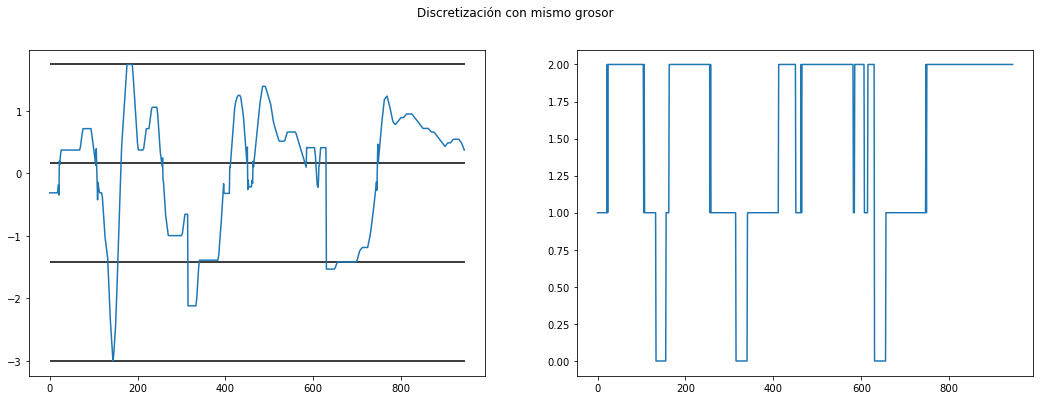
\includegraphics[width=1\textwidth]{ewd}
  \caption{Serie continua con 3 intervalos de mismo grosor (izquierda) y la serie discretizada (derecha).}
  \label{fig:ewd}
\end{figure}

Se utiliza la implementación de \emph{sklearn} en \emph{Python} con la clase \emph{KBinsDiscretizer}, usando el parámetro \emph{strategy = uniform}.

\section{Discretización con misma frecuencia}

La \textbf{discretización con misma frecuencia} realiza una idea parecida a la de mismo grosor pero en vez de dividir el rango de valores de la serie en $k$ contenedores se considera que cada contenedor tenga el mismo número de valores, es decir, la misma \textbf{frecuencia} (\autoref{def:efd}).

\begin{definicion}[Discretización con misma frecuencia]
  Sea una serie temporal continua $\{x_t\}_{t = 1}^n \subset I$  siendo $I$ un intervalo, el método de discretización con misma frecuencia en $k$ contenedores transforma la serie $\{x_t\}$ en una serie discreta $\{y_t\}_{t = 1}^n$ definida para $t = 1, \ldots n$, como:

  $$y_t = i-1, \; \text{ tal que } \; x_t \in I_i,$$

  donde $I = \cup_{i = 1}^k I_i$ y $\ell(I_i) = \frac{n}{k}, \, i = 1, \ldots, k$.
  \label{def:efd}
\end{definicion}

Creamos los contenedores realizando una partición del rango de valores de manera que cada uno tiene la misma frecuencia, o lo que es lo mismo, cada uno tiene $\frac{n}{k}$ observaciones.

En \autoref{fig:efd} mostramos un ejemplo de una serie continua discretizada en 3 contenedores con misma frecuencia, añadiendo los límites de los contenedores.

\begin{figure}[htpb]
  \centering
  %\hspace*{-2.5cm}
  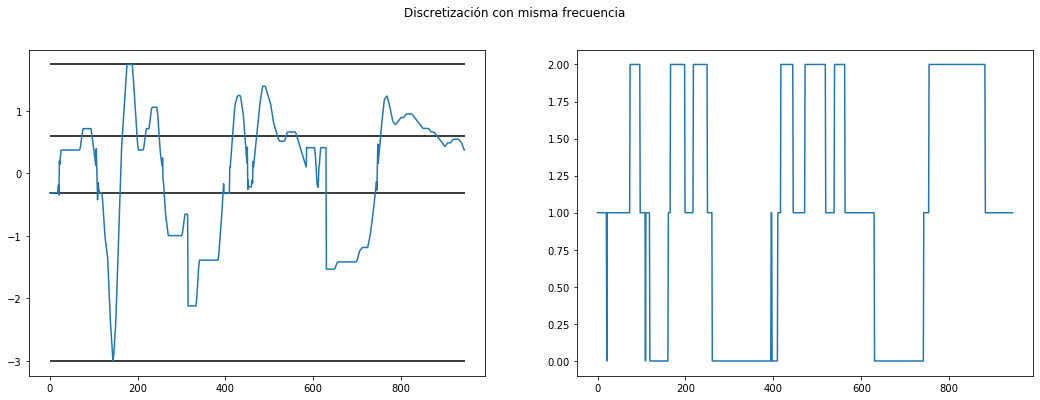
\includegraphics[width=1\textwidth]{efd}
  \caption{Serie continua con 3 intervalos de misma frecuencia (izquierda) y la serie discretizada (derecha).}
  \label{fig:efd}
\end{figure}

Se utiliza la implementación de \emph{sklearn} en \emph{Python} con la clase \emph{KBinsDiscretizer}, usando el parámetro \emph{strategy = quantile}.

\section{$k$-medias}

El algoritmo de $k$-medias (\emph{$k$-means}) \cite{macqueen1967some} es un algoritmo muy famoso y utilizado como método no supervisado de agrupamiento (\emph{clustering}) para poder dividir un conjunto de datos genérico en $k$ grupos donde se espera que cada grupo (\emph{cluster}) comparte unas características comunes.

Cada grupo está representado por un \textbf{centroide} de manera que a cada dato se le asigna al grupo cuyo centroide esté más cerca respecto la distancia euclidea (\autoref{def:k-means}).

\begin{definicion}[$k$-medias]
  Sea la matriz de datos $X = \begin{bmatrix} \textbf{x}_1 & \cdots & \textbf{x}_m \end{bmatrix}^T$ donde $\textbf{x}_i \in \R^n, \, i = 1, \ldots m$. El objetivo del algoritmo de $k$-medias es particionar los $m$ datos en $k$ grupos determinados por sus centroides $\textbf{C} = \{\pmb{\mu}_1, \ldots, \pmb{\mu}_k\}$ de manera que se minimize la inercia definida por

  $$\sum \limits^m_{i = 0} \min \limits_{\pmb{\mu} \in C} \left(||\textbf{x}_i - \pmb\mu ||^2 \right).$$
  \label{def:k-means}
\end{definicion}

En \autoref{fig:kmeans} \cite{ruiz2018kmeans} mostramos un ejemplo con datos con dos características (2D) aplicando $k$-medias con $k = 3$. Observamos que se obtienen 3 grupos con características similares.

\begin{figure}[htpb]
  \centering
  %\hspace*{-2.5cm}
  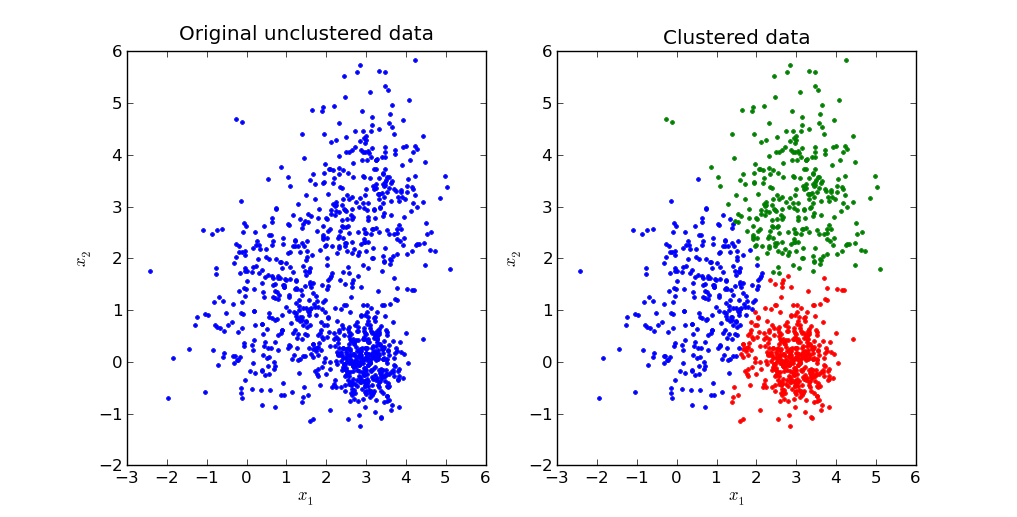
\includegraphics[width=1\textwidth]{kmeans}
  \caption{Ejemplo del algoritmo $k$-medias con $k=3$ aplicado a unos datos con 2 características (izquierda) del que se obtienen 3 grupos (derecha).}
  \label{fig:kmeans}
\end{figure}

Con este algoritmo obtenemos los $k$ contenedores como si fuesen los grupos representados por los centroides. Por tanto, cada punto se asigna al contenedor cuyo centroide esté más cerca (\autoref{def:kd}).

\begin{definicion}[Discretización con $k$-medias]
  Sea una serie temporal continua $\{x_t\}_{t = 1}^n$, el método de discretización con $k$-medias transforma la serie $\{x_t\}$ en una serie discreta $\{y_t\}_{t = 1}^n$ definida para $t = 1, \ldots, n$ como:

  $$y_t = i-1 \in N, \; \text{ tal que } \; i = \argmin \limits_{j = 1, \ldots, k} ||x_t - \pmb\mu_j||,$$

  donde $\pmb \mu_j$, $j = 1, \ldots, k$ son los centroides obtenidos en el algoritmo de $k$-medias.
  \label{def:kd}
\end{definicion}

Este método es más interesante que los anteriores ya que agrupa mediante las características de los datos por lo que puede obtenerse una discretización más significativa.

En \autoref{fig:dk} mostramos un ejemplo de una serie continua discretizada en 3 grupos, añadiendo los límites de los contenedores.

\begin{figure}[htpb]
  \centering
  %\hspace*{-2.5cm}
  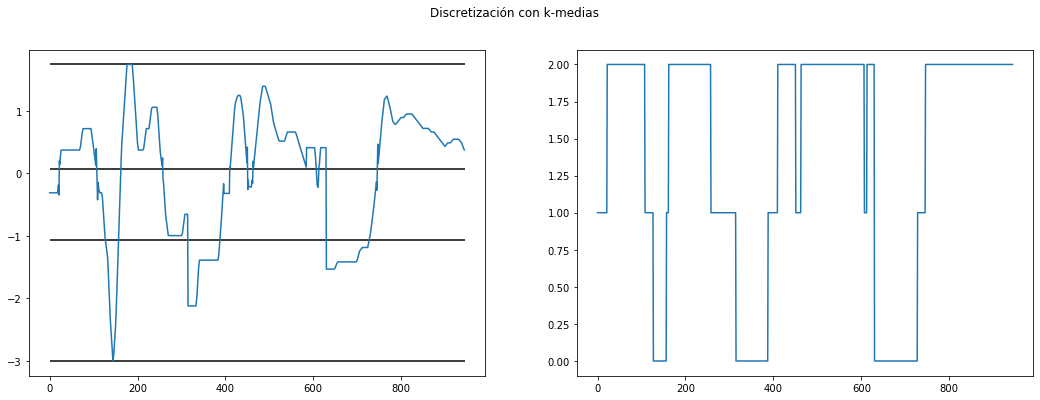
\includegraphics[width=1\textwidth]{dk}
  \caption{Serie continua con 3 intervalos de $k$-medias (izquierda) y la serie discretizada (derecha).}
  \label{fig:dk}
\end{figure}


Se utiliza la implementación de \emph{sklearn} en \emph{Python} con la clase \emph{KBinsDiscretizer}, usando el parámetro \emph{strategy = kmeans}.

\section{SAX}

El último método que desarrollamos es \emph{Symbolic Aggregate Aproximation} (SAX) \cite{lin2007experiencing}, un método más avanzado diseñado específicamente para series temporales. Este método transforma las series temporales en palabras de longitud igual o menor que las originales, permitiendo una discretización simbólica y una reducción de la dimensión.

Se necesitan indicar el número $k$ de contenedores que se codifican como una palabra de un alfabeto de tamaño $k$ (tomamos las $k$ primeras letras del abecedario latino) y el tamaño de ventana $w$ para dividir la serie en $\frac{n}{w}$ ventanas.

El algoritmo tiene tres pasos fundamentales: primero se toma la serie original y se normaliza (media 0 y varianza 1) (\autoref{def:normalizacion}).

\begin{definicion}[Normalización]
  Sea una serie temporal $\{x_t\}_{t = 1}^n$, su serie normalizada $\{s_t\}_{t = 1}^n$ está definida de la siguiente forma para $t = 1, \ldots, n$:

  $$s_t = \dfrac{x_t - \overline{x}}{\sigma_x},$$

  donde $\overline{x}$ es le media de la serie y $\sigma_x$ la desviación típica de la serie.
  \label{def:normalizacion}
\end{definicion}

Después se aplica a la serie normalizada una reducción de dimensión mediante el método PAA (\emph{Piecewise Aggregate Approximation}) \cite{keogh2001dimensionality} (\autoref{def:paa}).

\begin{definicion}[PAA]
  Sea una serie temporal $\{x_t\}_{t = 1}^n$ y un tamaño de ventana $w$, el método PAA reduce la dimensión de la serie transformándola en una serie de longitud $m = \frac{n}{w}$ denotado $\{\overline{x}_t\}_{t = 1}^m$ determinado por la siguiente expresión para $t = 1, \ldots, m$:

  $$\overline{x}_t = \dfrac{1}{n} \sum \limits_{i = (t-1)w + 1}^{tw} x_i.$$
  \label{def:paa}
\end{definicion}

Este método reduce la dimensión de la serie dividiendo en $m$ ventanas la serie normalizada y tomando la media de cada uno de ellos. En \autoref{fig:paa} mostramos un ejemplo de PAA con un tamaño de ventana $w$ de 157.

\begin{figure}[htpb]
  \centering
  %\hspace*{-2.5cm}
  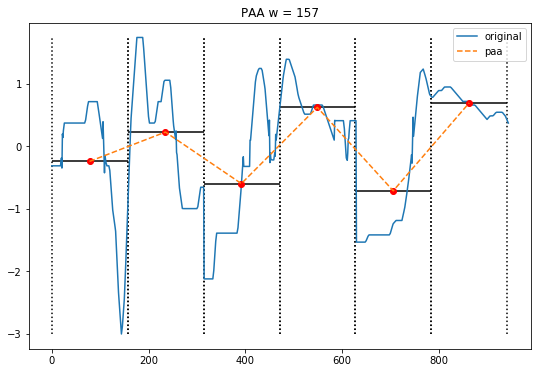
\includegraphics[width=.55\textwidth]{paa}
  \caption{Método PAA aplicado a una serie temporal con $w = 157$.}
  \label{fig:paa}
\end{figure}

Finalmente, aplicamos una discretización de la serie obtenida del método PAA asignando a cada ventana una letra de un alfabeto siendo generalmente el subalfabeto formado por los $k$ primeras letras del alfabeto latino.

La asignación de las letras se realiza de una manera similar a las técnicas descritas anteriormente, dividiendo el rango de valores en contenedores a los que se asigna una letra para cada uno. En este caso se divide la función de densidad de una distribución normal de manera que cada contenedor tiene el mismo área bajo la curva (\autoref{def:sax}).

\begin{definicion}[SAX]
  Sea una serie temporal $\{x_t\}_{t = 1}^n$ y un alfabeto de tamaño $k$ denotado por $A = \{a_1, \ldots, a_k\}$ el método SAX asigna a la serie una palabra $w = \alpha_1\alpha_2\ldots\alpha_n$, $\alpha_t \in A, \, t = 1, \ldots, n$ de la siguiente manera para $t = 1, \ldots n$:

  $$\alpha_t = a_i, \; \text{ si } \; \beta_{i-1} \leq x_t < \beta_i.$$

  donde $\beta_i$, $i = 1, \ldots n$, llamados puntos de ruptura (\emph{breakpoints}), son los valores tales que el área debajo de la curva de una distribución normal $N(0,1)$ desde $\beta_i$ hasta $\beta_{i+1}$ es $\frac{1}{k}$, $i = 1, \ldots n-1$.
  \label{def:sax}
\end{definicion}

Utilizando la función inversa de distribución acumulada podemos obtener fácilmente estos puntos de ruptura para cualquier $k$. En \autoref{fig:sax} \cite{lin2007experiencing} mostramos un ejemplo de como SAX transforma una serie temporal continua en la palabra \textbf{baabccbc}.

\begin{figure}[htpb]
  \centering
  %\hspace*{-2.5cm}
  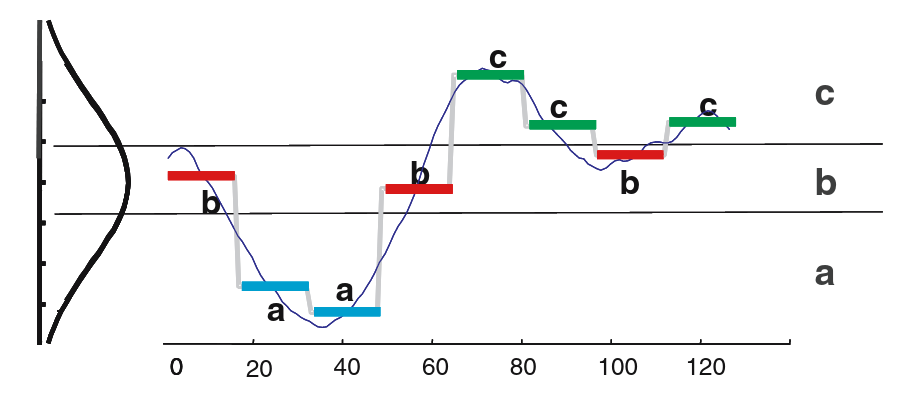
\includegraphics[width=.85\textwidth]{sax}
  \caption{Método SAX aplicado a una serie temporal con $w = 16$ y $k = 3$. Se aplica el método PAA y a cada sección se le asigna una letra.}
  \label{fig:sax}
\end{figure}

Se ha implementado la clase \emph{SAX} en \emph{Python} que ejecuta el método SAX y PAA en una versión basada para usar con la biblioteca \emph{sklearn}.

Cabe mencionar que aunque SAX transforme la serie en una palabra, podemos codificar cada letra como un número entero y poder trabajar con valores numéricos. Para ello se ha implementado también la clase \emph{DiscretizationEncoder} que usado junto con la clase \emph{SAX} nos permite hacer la codificación de las letras a numeros enteros.
